\documentclass[../main.tex]{memoir}

\begin{document}

\chapter{Análisis Didáctico}
\label{sec:analisis-didactico}

El conocimiento de los conceptos matemáticos por parte del profesor no garantizan la correcta enseñanza de los mismos. Es necesario un análisis profundo donde, por una parte, se analicen los contenidos a enseñar y su organización; por otra, la situación del alumnado. La unión de estas dos circunstancias guiará al profesor en la elección y diseño de actividades propicias y de un buen método de evaluación. En definitiva, es necesario llevar  a cabo un análisis didáctico. Segun \cite{rico2016}, el análisis didáctico es \textit{``el sistema y método de trabajo para el profesor de matemáticas, entre cuyas funciones destaca la reflexión sobre la estructura del currículo de matemáticas, junto con un dominio técnico para planificar e implementar unidades matemáticas escolares''.} \\

En esta sección, abordamos el Análisis de Contenidos, que estudia el sentido de los contenidos y su organización; el Análisis Cognitivo, que se centra en el aprendizaje de un tema matemático por parte de los estudiantes; el Análisis de Instrucción, en el que se deciden y diseñan ejercicios idóneos para el aprendizaje de los contenidos; y el Análisis Evaluativo, como pieza clave para la aplicación de un adecuado sistema de evaluación de lo aprendido.

\section{Análisis de Contenidos}

¿Qué es conocer un concepto matemático? Según \cite{rico2016}, \textit{``conocer su definición, representarlo, mostrar sus operaciones, relaciones y propiedades y los modos de uso, interpretación y aplicación a la resolución de problemas''.} Podemos llevar a cabo este conocimiento por dos vías. La primera, en la que aunamos la estructura conceptual y sus sistemas de representación, generan un significado instrumental del concepto, logrando su dominio por medio de un aprendizaje basado en la memorización de hechos, destrezas y propiedades. Por otra parte, se le puede dar un enfoque funcional, basado en que los conceptos y procedimientos asociados tienen una función y se usan con determinados propósitos. En definitiva, las diversas formas de entender, expresar y usar un concepto constituyen su significado. Por contenido matemático escolarse se entiende un conjunto de conceptos, procedimientos, estructuras y actitudes que los responsables del currículo escogen y organizan, que los profesores comunican y enseñan, para que los escolares aprendan acerca de un tópico matemático escolar determinado y lo utilicen. El análisis del contenido matemático escolar consiste en establecer con detalle sus descriptores y componentes particulares según cada una de las categorías cognitivas de contenido,establecidas por ámbitos y niveles. (\cite{rico2016}). \\

Este análisis se organiza en torno a tres aspectos:

\begin{itemize}
	\item Estructura conceptual. Se relacionan conceptos, procedimientos y actitudes implicados en el contenido objeto de estudio.
	\item Sistemas de Representación. Distintos modos de representación de un concepto matemático de acuerdo a su estructura o sus propiedades.
	\item Sentido. El análisis de contenido se ocupa de estudiar el sentido de un concepto matemático escolar analizando sus términos, contextos, fenómenos y situaciones en lo que se aplica.
\end{itemize}


\subsection{Estructura conceptual}

Según \cite{rico2016}, llamamos \textit{``estructura conceptual al primero de los sistemas de categorías u organizadores que identifica los aspectos formales y los cognitivos con que se caracterizan y describen los contenidos cuyo estudio se considera''}. Como ya comentamos antes, la estructura conceptual se divide en conceptos, procedimientos y actitudes. \cite{rico1997} indica que los conceptos son la sustancia general del conocimiento, aquello que pensamos, mientras que los procedimientos aglutinan los modos actuación y ejecución de tareas matemáticas. Finalmente, el campo actitudinal incluye los aspectos afectivos, éticos y normativos de la disciplina (\cite{rico2016}). Recuperando los contenidos de nuestra unidad didáctica (Real Decreto 1105/2014)

\begin{itemize}
	\item Números complejos
	\item Forma binómica y polar
	\item Representaciones gráficas
	\item Operaciones elementales
	\item Fórmula de Moivre.
\end{itemize}

\begin{table}[H]
	\centering
	\begin{tabular}{lcccccc}
		\toprule
		\hspace{2.5cm}Contenido conceptual \\
		\midrule
		- Parte real, parte imaginaria. Unidad imaginaria \\
		- Forma binómica \\
		- Afijo, módulo y argumento de un número complejo \\
		- Conjugado de un número complejo \\
		- Eje real y Eje Imaginario \\
		- Forma polar \\
		- Forma trigonométrica\\
		\bottomrule
	\end{tabular}
	\caption{Conceptos}
	\label{tab:conceptos}
\end{table}


\begin{table}[H]
	\centering
	\begin{tabular}{lcccccccccccc}
		\toprule
		\hspace{4cm}Contenido procedimental \\
		\midrule
		- Identificar la parte real y parte imaginaria de un número complejo \\
		- Calcular el afijo, módulo y argumento de un número complejo \\
		- Calcular el conjugado de un número complejo \\
		- Representar números complejos en su forma binómica y polar\\
		\hspace{0.2cm} en el plano complejo (Eje Real y Eje Imaginario) \\
		- Pasar de forma binómica a forma polar \\
		- Pasar de forma binómica y polar a forma trigonométrica\\
		- Operaciones con números complejos en forma binómica: sumar, \\ \hspace{0.2cm}multiplicar y dividir números complejos. Producto por escalar y potencia. \\
		- Operaciones con números complejos en forma polar: Producto, \\
		\hspace{0.2cm}división, raíz $n$-ésima y potencia. Uso de la fórmula de Moivre.\\
		\bottomrule
	\end{tabular}
	\caption{Procedimientos}
	\label{tab:procedimientos}
\end{table}

\begin{table}[H]
	\centering
	\begin{tabular}{lccccc}
		\toprule
		\hspace{4cm}Contenido actitudinal \\
		\midrule
		- Valoración del cuerpo de los números complejos como el conjunto \\ \hspace{0.2cm} numérico que engloba a los conocidos anteriormente ($\mathbb{N}, \mathbb{Z}, \mathbb{Q}, \mathbb{R}$). \\
		- Valoración de la importancia de los números complejos en ciencia y \\ \hspace{0.2cm} tecnología como en la física cuántica, circuitos electrónicos, \\ \hspace{0.2cm} electromagnetismo o dinámica de fluidos. \\
		\bottomrule
	\end{tabular}
	\caption{Actitudes}
	\label{tab:actitudes}
\end{table}


A su vez, cada concepto relacionada y organiza \textbf{hechos}. Se pueden entender como unidades de información que constituyen un primer nivel básico para analizar el ámbito conceptual de un contenido matemático. El estudio de los hechos se hace mediante cuatro categorías: términos, notaciones, convenios y resultados. Los hechos se relacionan y organizan para dar lugar a \textbf{conceptos} y \textbf{estructuras} (\cite{rico2016}). \\



Concretamente,

\begin{table}[H]
	\centering
	\begin{tabular}{llccccccccccccccccccccc}
		\toprule
		\hspace{5.5cm}\textbf{Hechos} \\
		\midrule
		Términos & Notaciones \\
		\midrule
		- Número complejo & - Forma binómica: $z = a +bi$, $\mathbb{C}$ \\
		& - $i$ unidad imaginaria \\
		- Parte real & - Re $z$ \\
		- Parte imaginaria & - Im $z$ \\
		- Afijo & - $P(a,b)$ punto del plano complejo\\
		- Módulo & - $|z|$ \\
		- Argumento & - $Arg z$ \\
		- Eje real, eje imaginario & \\
		 & - Conjugado: $\bar{z}$ \\
		 & - Forma polar: $z = r_\alpha$ \\
		\midrule
		Convenios & Resultados \\
		\midrule
		- El número complejo $z = a +bi$  & - Todo número complejo $z = a +bi$ \\
		se lee ``a más b i'', eludiéndose & se define como un punto $P(a,b)$  \\
		el signo de multiplicación. & del plano complejo  \\
		- Si $a=0, z$ se dice imaginario puro & - El eje real es el eje de abscisa y el eje \\
		&  imaginario es el eje de ordenadas. \\
		& Los números reales son números  \\
		& complejos con parte imaginaria  \\
		& nula ($b=0$) \\
		\bottomrule
	\end{tabular}
	\caption{Contenido conceptual: Hechos. Términos, notaciones, convenios y resultados}
	\label{tab:terminos-notaciones}
\end{table}


\begin{table}[H]
	\centering
	\begin{tabular}{lccccc}
		\toprule
		\hspace{2cm}Conceptos \\
		\midrule
		- Forma binómica \\
		- Forma polar \\
		- Forma trigonométrica\\
		- Raíz compleja de un polinomio \\
		\bottomrule
	\end{tabular}
	\caption{Contenido conceptual: Conceptos}
	\label{tab:conceptos2}
\end{table}

\begin{table}[H]
	\centering
	\begin{tabular}{lcc}
		\toprule
		\hspace{2.5cm}Estructuras \\
		\midrule
		 - ($\mathbb{C}$,+,·): Cuerpo de los números complejos \\
		\bottomrule
	\end{tabular}
	\caption{Contenido conceptual: Estructuras}
	\label{tab:estructuras}
\end{table}



Por otra parte, en el campo procedimental se diferencian, igualmente, tres niveles, según la complejidad del contenido. Son las destrezas, que procesan hechos; los razonamientos, que procesan conceptos; y las estrategias, que procesan estructuras (\cite{rico2016}). \\

\begin{table}[H]
	\centering
	\begin{tabular}{lcccccc}
		\toprule
		\hspace{5.5cm}Destrezas \\
		\midrule
		- Identificar la parte real y parte imaginaria de un número complejo \\
		- Calcular el afijo, módulo y argumento de un número complejo \\
		- Calcular el conjugado de un número complejo \\
		- Representar números complejos en su forma binómica y polar\\
		\hspace{0.2cm} en el plano complejo (Eje Real y Eje Imaginario) \\
		\bottomrule
	\end{tabular}
	\caption{Contenido procedimental: Destrezas}
	\label{tab:destrezas}
\end{table}


\begin{table}[H]
	\centering
	\begin{tabular}{lcccccc}
		\toprule
		\hspace{5.5cm}Razonamientos \\
		\midrule
		- Pasar de forma binómica a forma polar \\
		- Pasar de forma binómica y polar a forma trigonométrica\\
		- Operaciones con números complejos en forma binómica: sumar, \\ \hspace{0.2cm}multiplicar y dividir números complejos. Producto por escalar y potencia. \\
		- Operaciones con números complejos en forma polar: Producto, \\
		\hspace{0.2cm}división, raíz $n$-ésima y potencia. Uso de la fórmula de Moivre.\\
		\bottomrule
	\end{tabular}
	\caption{Contenido procedimental: Razonamientos}
	\label{tab:razonamientos}
\end{table}


%% PREGUNTAR POR ESTRATEGIAS
\begin{table}[H]
	\centering
	\begin{tabular}{lcccccc}
		\toprule
		\hspace{5.5cm}Estrategias \\
		\midrule
		\bottomrule
	\end{tabular}
	\caption{Contenido procedimental: Estrategias}
	\label{tab:estrategias}
\end{table}


%% MAPA CONCEPTUAL --> PREGUNTAR

\subsection{Sistemas de Representación}

Comprender un concepto matemático, o una estructura en su totalidad, requiere que el alumno lo recree en su mente por medio de imágenes o representaciones más o menos abstractas. Dichas representaciones deben ser lo más ricas y variadas posibles, para así garantizar la correcta interpretación y captar, en sentido amplio, la naturaleza del concepto objeto de estudio. Concretamente, según \cite{rico2016}, un sistema de representación \textit{``constituye un conjunto estructurado de notaciones, símbolos y gráficas, dotado de una serie de reglas y convenios que permiten expresar determinados aspectos y propiedades de un concepto matemático''}. Por su parte, \cite{lupi2013} señala que cada sistema de representación destaca alguna peculiaridad del concepto que expresa y facilita el entendimiento y trabajo de alguna de sus propiedades. Por todo ello, proponemos cuatro sistemas de representación distintos en torno a un número complejo. Son las siguientes: representación numérica, simbólica o algebraica, representación verbal, representación gráfica y la representación por medio de recursos digitales. 

\subsubsection{Representación numérica, simbólica o algebraica}

En primer lugar, entendemos el cuerpo de los número complejos, $\mathbb{C}$, simbólicamente como 

$$\mathbb{C} \{a+bi, \forall a,b \in \mathbb{R}\}$$

siendo $i = \sqrt{-1}$. Por tanto, todo número complejo $z$, dados $a,b \in \mathbb{R}$, se puede expresar como

$$z = a+bi, \hspace{1cm} \text{Re }z = a, \text{ Im }z = b$$

Esta representación es llamada forma binómica de un número complejo. No obstante, los números complejos se pueden representar simbólicamente de otras formas. Si llamamos $r = |z|$ y $\alpha = $ Arg $z$, entonces $z = r_{\alpha}$ (forma polar o módulo-argumental de un número complejo). \\

Finalmente, dada la forma binómica y polar, si $a = r \cos \alpha, b=r \sin \alpha$, la forma trigonométrica de un número complejo $z$ se escribe como

$$ z = a + bi = r \cos \alpha + (r \sin \alpha) i = r(\cos \alpha + i \sin \alpha)$$

\subsubsection{Representación verbal}

Habitualmente, los números complejos (también conocidos como imaginarios) se representan verbalmente por medio de la lectura de su forma binómica. Tal y como se indicó en los convenios de la sección anterior, el signo de multiplicación entre la parte imaginaria y la unidad imaginaria se obvia, por lo que, por ejemplo, para el número $z = 5+3i$, se representa verbalmente como ``cinco más tres i''. Por otra parte, se puede expresar el mismo número complejo a través de su forma polar indicando el módulo y argumento. En nuestro ejemplo, $z = \sqrt{34}_{30.96º}$ como ``número complejo con módulo raíz de 34 y argumento 30.96º''.

\subsubsection{Representación gráfica}

Todo número complejo se puede representar por medio del diagrama de Argand o plano complejo. Dada la similitud absoluta con $\mathbb{R}^2$ en cuanto a este aspecto, la representación gráfica es clave para la correcta comprensión por parte del alumno del bloque que nos ocupa. No obstante, también se puede utilizar otro tipo de representaciones para mostrar, por ejemplo, que todos los conjuntos numéricos conocidos son subconjunto del cuerpo de los números complejos. Es decir, que $\mathbb{N} \subset \mathbb{Z} \subset \mathbb{Q} \subset \mathbb{R} \subset \mathbb{C}$. 

\begin{figure}[hbtp]
	\centering
	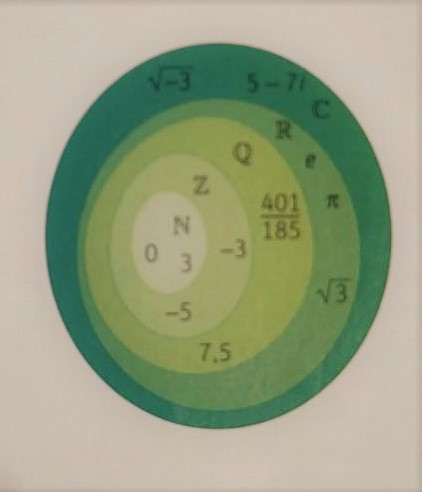
\includegraphics[width=\linewidth]{images/complex.jpg}
	\caption{$\mathbb{C}$ como un todo}
	\label{representacion1}
\end{figure}

Asimismo, presentamos el plano complejo o diagrama de Argand y la representación de un número complejo en forma binómica, mostrando su afijo, módulo y argumento.
\begin{figure}[hbtp]
	\centering
	\begin{subfigure}{0.48\textwidth}
		\centering
		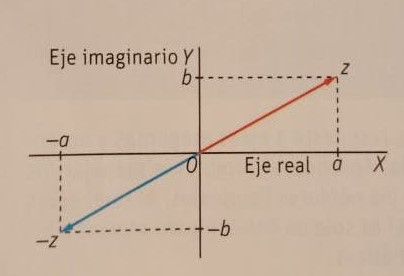
\includegraphics[width=\linewidth]{images/ejes.jpg}
		\caption{Eje Real y Eje Imaginario}
	\end{subfigure}
	\begin{subfigure}{0.48\textwidth}
		\centering
		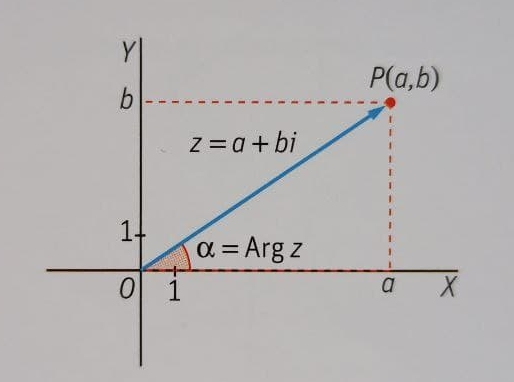
\includegraphics[width=\linewidth]{images/afijo.jpg}
		\caption{Afijo, módulo y argumento de un número complejo (forma binómica)}
	\end{subfigure}
	\label{fig:representacion2}
\end{figure}

Finalmente, representamos un número complejo en su forma polar y trigonométrica.

\begin{figure}[hbtp]
	\centering
	\begin{subfigure}{0.48\textwidth}
		\centering
		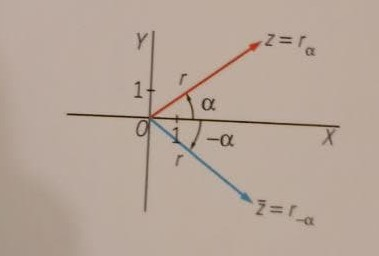
\includegraphics[width=\linewidth]{images/polar.jpg}
		\caption{Representación en forma polar}
	\end{subfigure}
	\begin{subfigure}{0.48\textwidth}
		\centering
		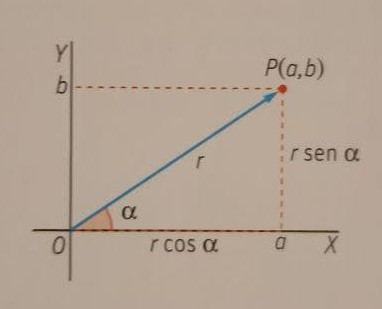
\includegraphics[width=\linewidth]{images/trigonometrica.jpg}
		\caption{Representación en forma trigonométrica}
	\end{subfigure}
	\label{fig:representacion3}
\end{figure}

\subsubsection{Recursos digitales}

\subsection{Sentido del Concepto Matemático}

\subsubsection{Términos}


\subsubsection{Contextos Matemáticos}

\subsubsection{Fenómenos}

Tal y como expresa \cite{lupi2013} en \cite{rico2013}, la historia es un buen mecanismo para estudiar el contenido de un tema, pues el desarrollo histórico es útil para determinar el origen de los conceptos, comparar sistemas de representación o localizar problemas clásicos.


\subsubsection{Situaciones}
\end{document}

%%% Local Variables:
%%% mode: latex
%%% TeX-master: "../main"
%%% End:
